\chapter{Netzwerke}

\section{Einführung}
Was geschieht, wenn Sie Ihren Freunden eine Nachricht schreiben? Ihre Freunde erhalten eine Benachrichtigung mit Ihrer Nachricht und können Ihnen darauf antworten. Was Ihnen möglicherweise weniger bewusst ist, sind die Schritte, die nötig sind, damit die Nachricht Ihren Weg von A (Ihnen) zu B (Ihren Freunden) findet und damit diese korrekt übermittelt wird. Vermutlich wissen Sie bereits, dass zwischen Ihrem Geräten und deren Ihrer Freunde das \textbf{Internet} liegt. Dieses Skript soll Ihnen ermöglichen, die Grundlagen des Internets zu verstehen.

Dazu müssen wir zuerst verstehen, was ein Netzwerk ist. Ein \textbf{Netzwerk} ist im Grunde genommen ein \textbf{Graph} aus \textbf{Knoten} und \textbf{Kanten}. Bevor wir uns die Grundlagen von Netzwerken anschauen, setzen wir uns daher zuerst mit Graphen auseinander.

\section{Graphen}
Graphen sind abstrakte Informationsdarstellungen, die uns erlauben, Informationen unterschiedlichster Arten darzustellen, darunter:
\begin{itemize}
    \item Verkehrsnetzwerke wie Strassen, Eisenbahnennetze etc., welche erlauben, Navigations-Apps oder Infrastrukturplanung zu betreiebn
    \item Datenstrukturen und Algorithmen in Computern, um vielerlei Probleme schneller und effizienter zu lösen
    \item Chemische Strukturen in der Medizin, um bessere Medikamente zu finden
\end{itemize}

Im Allgemeinen dienen Graphen in der Informatik \& Mathematik zur Darstellung Relationen zwischen Objekten beliebiger Art. \textbf{Relationen} sind dabei vereinfacht als Verhältnisse zwischen zwei Objekten zu verstehen, beispielsweise:
\begin{itemize}
\item Zug A fährt von Ort$_1$ nach Ort$_2$.
\item Person A lebt gemeinsam mit Person B
\item Atom A ist mit Atom B zu einem Molekül verbunden
\end{itemize}
Wie können solch unterschiedliche Informationen auf eine ähnliche, systematische und für den Computer verständliche Art dargestellt werden? Dazu lernen wir im Folgenden das Konzept von \textbf{Graphen} kennen.
\subsection{Graphen, Kanten und Knoten}
Ein \textbf{Graph} $G=(V,E)$ ist ein Paar von zwei Mengen $V$ und $E$
\begin{itemize}
    \item $V$ ist die \textbf{Menge der Knoten}. Diese werden gezeichnet als Punkte oder kleine Kreise. Alle Knoten haben Namen.
    \item $E$ ist die \tib{Menge der Kanten}. Die Kanten verbinden Knoten und werden Bezeichnet durch ihre Endknoten
\end{itemize}

Ein Beispiel eines einfachen Graphen ist gegeben in \cref{fig:graph-ex}.
\begin{figure}
    \centering
    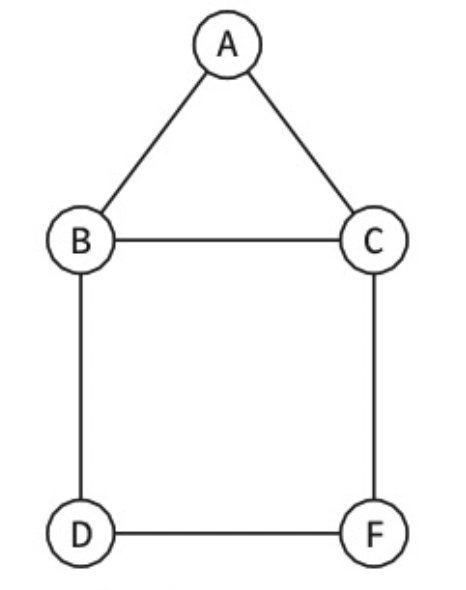
\includegraphics[keepaspectratio, width=0.22 \paperwidth]{GrundlagenInfo/02_Graphen/Figures/4-graph.png}
    \label{fig:graph-ex}
\end{figure}
Der Graph in \cref{fig:graph-ex} besteht aus folgenden Komponenten:
\begin{itemize}
    \item Knoten $V=\lrc{A,B,C,D,F}$
    \item Kanten $E=\lrc{\lrc{A,B},\lrc{A,C},\lrc{B,C},\lrc{B,D},\lrc{C,F},\lrc{D,F}}$
\end{itemize}
\subsection{Wege und Kreise in Graphen}
\begin{itemize}
    \item Ein \tib{Weg} oder ein \tib{Spaziergang} in einem Graphen $G=(V,E)$ besteht aus einer Folge benachbarter Knoten, die miteinander verbunden werden
    \begin{itemize}
        \item Z.B. im Graph unten: $A,B,C,F,D$
        \item Wir sagen dem ersten und letzten Knoten in diesem Weg ($A$ und $D$) \tib{Endknoten}
        \begin{figure}
            \centering
            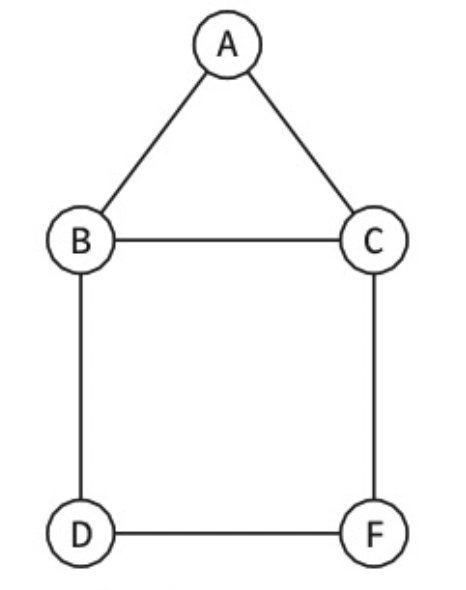
\includegraphics[keepaspectratio, width=0.2 \paperwidth]{GrundlagenInfo/02_Graphen/Figures/4-graph.png}
        \end{figure}
    \end{itemize}
    \item Wir nennen einen Weg \tib{Kreis}, wenn die Endknoten gleich sind
    \begin{itemize}
        \item Z.B. $A,C,F,D,B,A$
        \item Ein Kreis ist \tib{einfach}, wenn ausser dem Endknoten kein anderer Knoten zweimal vorkommt
    \end{itemize}
\end{itemize}

Dabei gibt es bestimmte spezielle Wege in Graphen:

Ein \tib{Euler'scher Weg} ist ein Weg, der alle Kanten eines Graphen genau einmal durchläuft. Graphen, die einen solchen Weg besitzen, nennen wir \tib{Euler'sche Graphen}

{Eulers Besuch in Königsberg}
\begin{itemize}
    \item Der berühmte Schweizer Mathematiker Leonhard Euler soll im Jahre 1736 die Stadt Königsberg besucht haben.
    \item Königsberg war damals die Hauptstadt der deutschen Provinz Ostpreussen.
    \item Seit dem Jahre 1946 gehört die Stadt zu Russland und wurde in \textit{Kaliningrad} unbenannt.
\end{itemize}

Der berühmte Schweizer Mathematiker Leonhard Euler soll im Jahre 1736 die Stadt Königsberg besucht haben. Königsberg war damals die Hauptstadt der deutschen Provinz Ostpreussen. Seit dem Jahre 1946 gehört die Stadt zu Russland und wurde in \textit{Kaliningrad} unbenannt. In \cref{fig:stadtplanCrop} sehen Sie den für uns relevanten Ausschnitt eines Stadtplans des damaligen Königsbergs.
\begin{figure}[H]
    \centering
    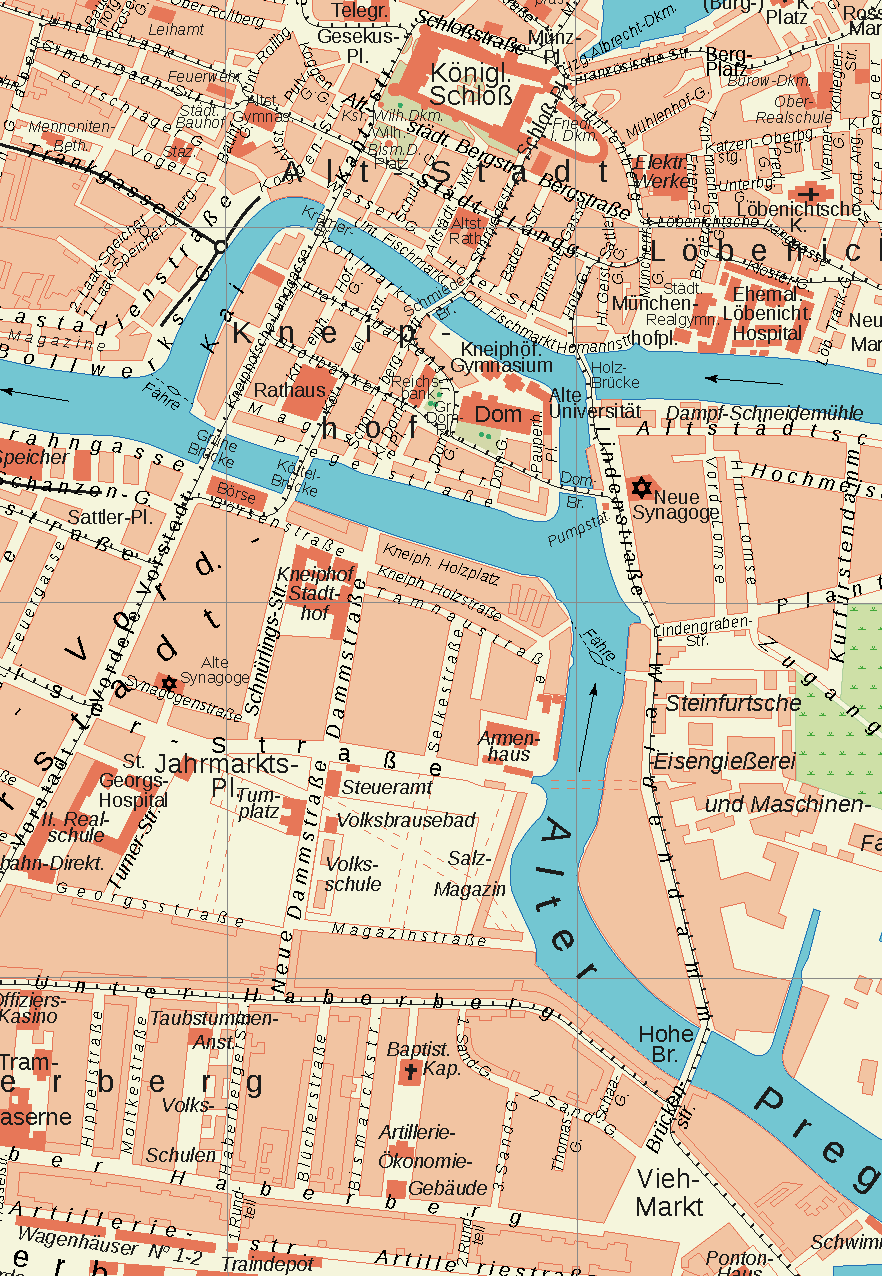
\includegraphics[width=0.5\textwidth]{GrundlagenInfo/02_Graphen/AbstraktionDurchGraphen/Figures/StadplanCrop.pdf}
    \caption{Ausschnitt aus einem Stadtplan des damaligen Königsbergs}
    \label{fig:stadtplanCrop}
\end{figure}
\noindent
In \cref{fig:stadtplanCropMitBuchstaben} haben wir die vier verschiedenen Stadtteile Kneiphof ($A$), Vorstadt ($B$), Alt-Stadt ($C$) und Lomse ($D$) sowie die sieben Brücken zwischen ihnen hervorgehoben. Die Stadtteile werden von dem Fluss \textit{Pregel} von einander getrennt.
\begin{figure}[H]
    \centering
    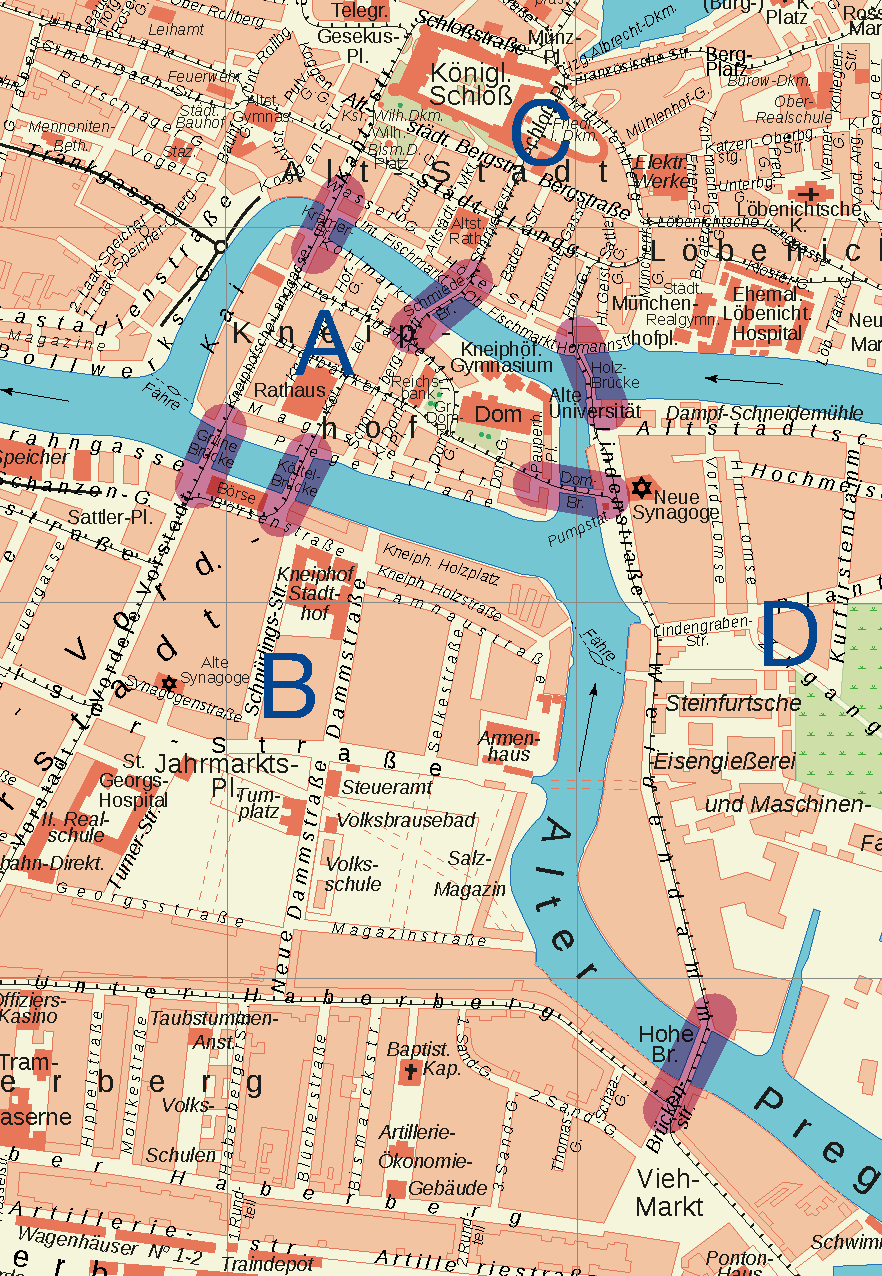
\includegraphics[width=0.5\textwidth]{GrundlagenInfo/02_Graphen/AbstraktionDurchGraphen/Figures/StadplanCropMitBuchstaben.pdf}
    \caption{die vier Stadtteile $A, B, C$ und $D$ von Königsberg verbunden durch sieben Brücken}
    \label{fig:stadtplanCropMitBuchstaben}
\end{figure}
\noindent
Der Legende nach kursierte unter den Spaziergängerinnen und Spaziergängern von Königsberg damals die folgende Frage, welche heute als \tib{Königsberger Brückenproblem} bekannt ist:
\begin{myexercise}[Königsberger Brückenproblem]\label{myBox:Problem}
Gibt es einen Weg durch Königsberg, bei dem man alle sieben Brücken \textbf{genau einmal} überquert, und wenn ja, ist auch ein Rundweg möglich, bei dem man wieder zum Ausgangspunkt gelangt?    
\end{myexercise}
\noindent
Euler realisierte vermutlich, dass es keine Rolle spielt, wie sich eine Spaziergängerin innerhalb eines Stadtteils bewegt. Relevant sind lediglich die Übergänge zwischen den Stadtteilen über die Brücken. Vermutlich abstrahierte er das Problem durch eine Skizze wie in \cref{fig:skizze}.

\begin{figure}[H]
    \centering
    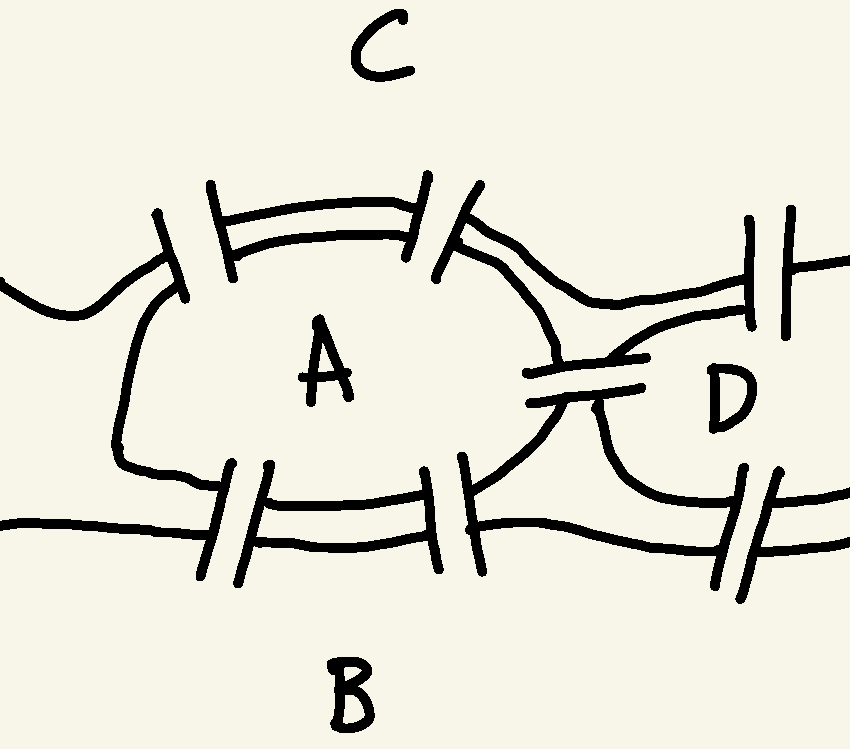
\includegraphics[width=0.3\textwidth]{GrundlagenInfo/02_Graphen/AbstraktionDurchGraphen/Figures/vonHandCrop.pdf}
    \caption{abstrakte Skizze von Königsberg}
    \label{fig:skizze}
\end{figure}
\noindent
Selbst diese Skizze kann noch weiter abstrahiert werden, ohne dass wir relevante Informationen für das Königsberger Brückenproblem verlieren. Beispielsweise brauchen wir den Fluss nicht darzustellen. Dabei könnte man zur Abstraktion in \cref{subfig:graph} gelangen.

%% Aufgabenblatt %%
\begin{figure}[H]
\centering

\begin{subfigure}[b]{0.4\textwidth}
\centering
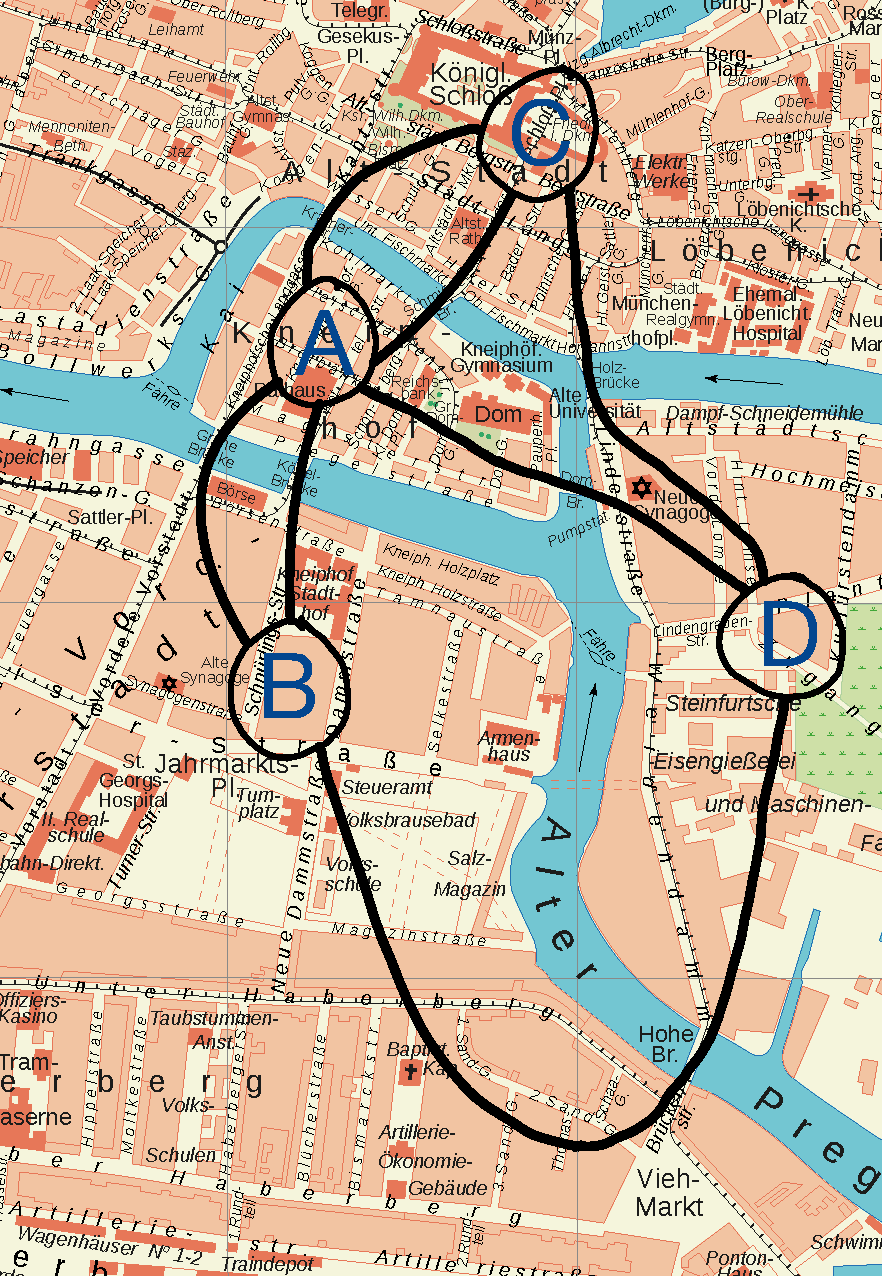
\includegraphics[width=0.9\textwidth]{GrundlagenInfo/02_Graphen/AbstraktionDurchGraphen/Figures/GraphAufStadtplan.pdf}
\caption{Stadtplan}
\end{subfigure}
\hfill
\begin{subfigure}[b]{0.4\textwidth}
\centering
\resizebox{0.7\textwidth}{!}{%
\begin{tikzpicture}[shorten >=1pt,auto,node distance=3cm, semithick, scale=0.25]
  \node[state] (A)              {$A$};
  \node[state] (B) [below of=A] {$B$};
  \node[state] (C) [above of=A] {$C$};
  \node[state] (D) [right of=A] {$D$};

  \path (A) edge [bend right] node {} (B)
        (A) edge [bend left] node {} (B)
        (A) edge [bend right] node {} (C)
        (A) edge [bend left] node {} (C)
        (A) edge node {} (D)
        (B) edge node {} (D)
        (C) edge node {} (D);
\end{tikzpicture}
}%
\caption{Darstellung als Graph}
\label{subfig:graph}
\end{subfigure}
\caption{Modellierung des Königsberger Brückenproblems durch einen Graphen mit vier Knoten und sieben Kanten}
\label{fig:EulerGraph}
\end{figure}

\noindent
Die schematische Darstellung in \cref{subfig:graph} ist lediglich ein Modell der eigentlichen Situation in Königsberg. Allerdings enthält dieses Modell sämtliche für das Problem relevanten Teile und lässt alle nicht relevanten Teile geschickt weg. Das Modell stellt also eine hervorragende Abstraktion des Problems dar. Eine solche Art der Abstraktion wie in \cref{subfig:graph}  wird \tib{Graph} genannt.



Ein \tib{Hamilton'scher Weg} ist ein einfacher Weg zwischen zwei Knoten eines Graphen, bei dem alle Knoten des Graphen enthalten sind.

\begin{myexercise}
Suchen Sie Euler'sche Wege/Kreise und Hamilton'sche Wege/Kreise im Graph aus \cref{fig:graph-ex}.
\end{myexercise}
   

\section{Netzwerke}

\section{Das Internet}


\begin{figure}[H]
\centering
\begin{tikzpicture}[
    auto,
    block/.style={
	    minimum width=3cm,
	    node distance=1.5cm,
        rectangle, 
        fill=RoyalBlue!50, 
        align=center, 
        rounded corners
    }
]


% Define the nodes with FontAwesome icons
\node[block] (chefs) {\faFemale\ Chef};
\node[block, below=of chefs] (secretariat) {\faPhone\ Sekretariat};
\node[block, below=of secretariat] (postman) {\faMale\ Post};


% Define the nodes with FontAwesome icons

\node[block, right=of postman] (postman2) {\faMale\ Post};
\node[block, above=of postman2] (secretariat2) {\faPhone\ Sekretariat};
\node[block, above=of secretariat2] (chefs2) {\faMale\ Chef};


% Draw the dashed arrows
\draw[<->, dashed, RoyalBlue!50, thick] (chefs) -- (chefs2);
\draw[<->, dashed, RoyalBlue!50, thick] (secretariat) -- (secretariat2);
\draw[<->, dashed, RoyalBlue!50, thick] (postman) -- (postman2);

\draw[->, line width=1mm,ForestGreen!50] (chefs) -- node[left]{\faComments} (secretariat) ;
\draw[->, line width=1mm,ForestGreen!50] (secretariat) -- node[left]{\faEnvelope} (postman) ;
\draw[->, line width=1mm,ForestGreen!50, bend right] (postman.south) to node[midway,below]{\faBicycle\ \faMotorcycle\ \faCar\ \faShip\ \faPlane} (postman2.south) ;
\draw[->, line width=1mm,ForestGreen!50] (postman2) -- node[right]{\faEnvelope} (secretariat2) ;
\draw[->, line width=1mm,ForestGreen!50] (secretariat2) -- node[right]{\faComments} (chefs2) ;

% fit rectangles around regions
\node[fit=(chefs) (postman), inner sep=8pt, red, dotted, draw, line width=1pt,rounded corners](region1) {};
\node[fit=(chefs2) (postman2), inner sep=8pt, red, dotted, draw, line width=1pt,rounded corners](region2) {};
% annotate both rectangles
\node[above=5pt of region1.north, anchor=center, align=center]{\textcolor{red}{Firma 1, Europa}};
\node[above=5pt of region2.north, anchor=center, align=center]{\textcolor{red}{Firma 2, Asien}};

\end{tikzpicture}
\end{figure}